\section{Ejercicio 3: El retorno del jedi}

    % Describir detalladamente el problema a resolver dando ejemplos del mismo y sus soluciones.
    \subsection{Descripción del problema}

	Luke debe enfrentar a su padre. Para ello debe moverse por una grilla,
	arrancando en la esquina superior izquierda para terminar en la opuesta,
	donde aguarda Darth Vader. Cada casilla de la grilla tiene una altura
	asociada, donde dependiendo de la diferencia en altura entre el casillero
	actual de Luke y su destino le costará más o menos energía moverse. Además
	se tiene la condición de que Luke únicamente puede avanzar hacia abajo o
	hacia la derecha, dado que considera un acto de cobardía retroceder sobre
	sus pasos. El objetivo es encontrar y devolver el camino donde Luke gasta la
	menor cantidad de energía en alcanzar su destino.

	Formalizando el problema, se tiene una grilla $G$ rectangular de dimensiones $N \times
	M$ donde Luke comienza en la posición $(1, 1)$ y desea llegar a $(N, M)$.
	Sea $G_{ij}$ con $1 \leq i \leq N$ y $1 \leq j \leq M$ la altura de cada
	casillero, $H$ el nivel de entrenamiento de Luke y $\Delta$ la
	diferencia de altura entre el casillero actual y el próximo, el costo de
	energía para cada movimiento se calcula de la siguiente manera: nulo si $|\Delta|
	\leq H$, $|\Delta| - H$ en caso contrario. La condición de que Luke no pueda
	retroceder es equivalente a decir que únicamente puede moverse de forma
	creciente en $i$ o $j$.

	El formato de entrada para el problema es el siguiente, donde la primer
	línea posée las dimensiones de la grilla y el nivel de entrenamiento de
	Luke, y las siguientes $N$ entradas contienen $M$ elementos donde cada uno
	representa la altura del casillero correspondiente.

	~

	\begin{tabular}{cccc}
		$N$ & $M$ & $H$ & \\
		$G_{11}$ & $G_{12}$ & $\dots$ & $G_{1M}$ \\
		$G_{21}$ & $G_{22}$ & $\dots$ & $G_{2M}$ \\
		$\vdots$ & & & \\
		$G_{N1}$ & $G_{N2}$ & $\dots$ & $G_{NM}$ \\
	\end{tabular}

	~

	La salida está compuesta por una primer línea con el costo del camino
	seleccionado y $N + M - 2$ líneas con la dirección ($X$ o $Y$) a tomar en cada paso para
	realizar el mismo. Cabe aclarar que $X$ implica un movimiento de filas e $Y$
	de columnas.

	A continuación se presenta un ejemplo de entrada con su salida
	correspondiente:

	~

	\begin{figure}[H]
		\centering
		\begin{minipage}[t]{0.25\textwidth}
			\begin{tabular}[t]{ccc}
				\multicolumn{3}{l}{\textbf{Entrada}} \\
				\texttt{3} & \texttt{3} & \texttt{1} \\
				\texttt{4} & \texttt{-2} & \texttt{-1} \\
				\texttt{6} & \texttt{7} & \texttt{-5} \\
				\texttt{0} & \texttt{3} & \texttt{4} \\
			\end{tabular}
		\end{minipage}
		\begin{minipage}[t]{0.10\textwidth}
			\begin{tabular}[t]{l}
				\textbf{Salida} \\
				\texttt{4} \\
				\texttt{X} \\
				\texttt{Y} \\
				\texttt{X} \\
				\texttt{Y} \\
			\end{tabular}
		\end{minipage}
	\end{figure}

	\begin{figure}[H]
		\centering
		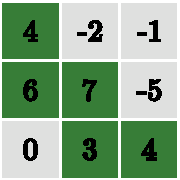
\includegraphics{imagenes/ej3_grilla_1.pdf}
		\caption{Camino de menor costo.}
	\end{figure}

    % Explicar de forma clara, sencilla, estructurada y concisa, las ideas desarrolladas para la resolución del problema. Utilizar pseudocódigo y lenguaje coloquial (no código fuente). Justificar por qué el procedimiento resuelve efectivamente el problema.
    \subsection{Solución propuesta}

    % Deducir una cota de complejidad temporal del algoritmo propuesto (en función de los parámetros que se consideren correctos) y justificar por qué el algoritmo la cumple. Utilizar el modelo uniforme.
    \subsection{Complejidad teórica}

    % Realizar experimentación para medir la performance, usando un conjunto de casos de test que permitan observar los tiempos de ejecución en función de los parámetros de entrada, tanto para instancias aleatorias (detallando cómo fueron generadas) como para instancias particulares (peor/mejor caso, por ejemplo). Presentar en forma gráfica una comparación entre los tiempos medidos y la complejidad teórica y extraer conclusiones.
    \subsection{Experimentación}

    % Ejemplo de gráfico para reutilizar:
    % \begin{figure}[H]
    %     \centering
    %     \caption{}
    %     \label{fig:exp1:tiempo_base}
    %     \begin{tikzpicture}
    %         \begin{axis}[
    %                 title={},
    %                 xlabel={Tamaño de entrada ($N$)},
    %                 ylabel={Tiempo de ejecución (nanosegundos)},
    %                 scaled x ticks=false,
    %                 scaled y ticks=false,
    %                 enlargelimits=0.05,
    %                 width=0.5\textwidth,
    %                 height=0.5\textwidth,
    %                 legend pos=south east,
    %                 legend cell align=left,
    %                 xmin=1
    %             ]
    %             \addplot[color=black] table[x index=0,y index=1]{../exp/kaioKenOutput};
    %             \addplot[color=red] table[x index=0, y expr={x*ln(x)*\constante}]{../exp/kaioKenOutput};
    %             \legend{$T$, $c*N*log(N)$}
    %         \end{axis}
    %     \end{tikzpicture}
    % \end{figure}
